\thispagestyle{fancy}
\begin{center}
	\LARGE{\textbf{Ley de tensiones de Kirchhof}}
\end{center}
\section{Objetivos}
Al finalizar esta experiencia, usted estará capacitado para:
\begin{enumerate}
	\item Utilizar el multímetro para medir caídas de tensión en circuito en serie.
	\item Demostrar en circuitos serie la ley de las tensiones de Kirchhoff.
\end{enumerate}
\section{Conocimientos previos}
La ley de las tensiones de Kirchhoff establece que la suma algebraica de las tensiones en una malla cerrada es cero. Para utilizar esta ley, lija una malla cerrada
para analizar.
\\
Elija un punto de inicio. A partir del mismo, recorra la malla, terminando en el punto
donde comenzó.
\begin{figure}[h]
	\centering
	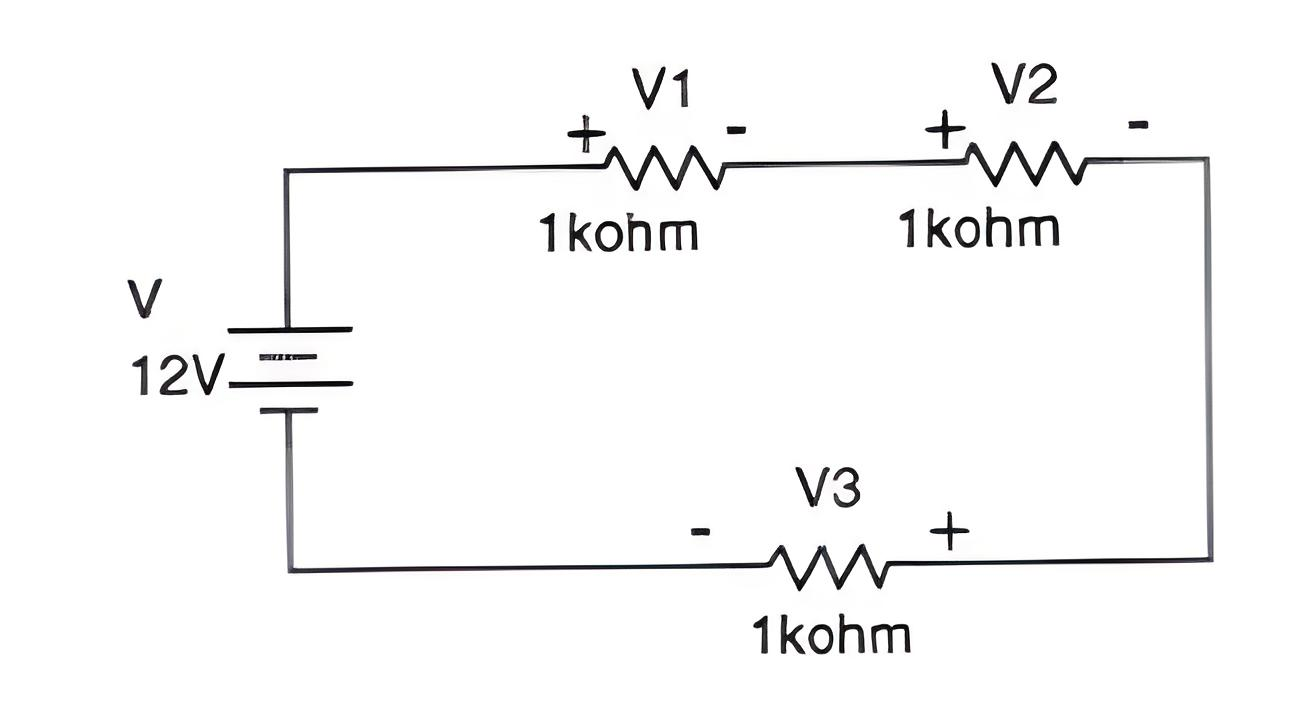
\includegraphics[scale=0.2]{imagenes/1}
\end{figure}
Siguiendo el recorrido de la malla, sume las caídas de tensión en cada componente. Si la tensión en el componente es positiva, la acompañara un signo "+", y si la tensión es negativa, la acompañara el signo "$\- $".\\
\begin{equation*}
	V_{1}+V_{2}+V_{3}-V=0
\end{equation*}
Cuando haya remplazado el recorrido, la suma de las caídas de tensión será 0.
\begin{equation*}
	\sum V=0
\end{equation*}
\section{Autoevaluación de entrada}
\begin{enumerate}
	\item Dos resistores s. 1 conectados en serio, se sabe que la caída de tensión en cada
	resistor es BV, por lo que la caída en ambos resistores es: diferente puesto que un circuito en serie el voltaje varia en cada resistencia dependiendo de la capacidad de un resistor
	\item  La suma algebraica de las caídas de tensión en una malla de un circuito cerrado es: igual 0 puesto que la suma de todos los voltajes de las resistencia es igual voltaje de la fuente.
\end{enumerate}
\section{Equipo}
El siguiente equipo para realizar la experiencia 
\begin{enumerate}
	\item Modulo experimental 
	\item DMM (digital)
\end{enumerate}
\section{Procedimiento}
\begin{enumerate}
	\item Efectué los cálculos correspondientes para el circuito de la figura.
	\begin{figure}[h]
		\centering
		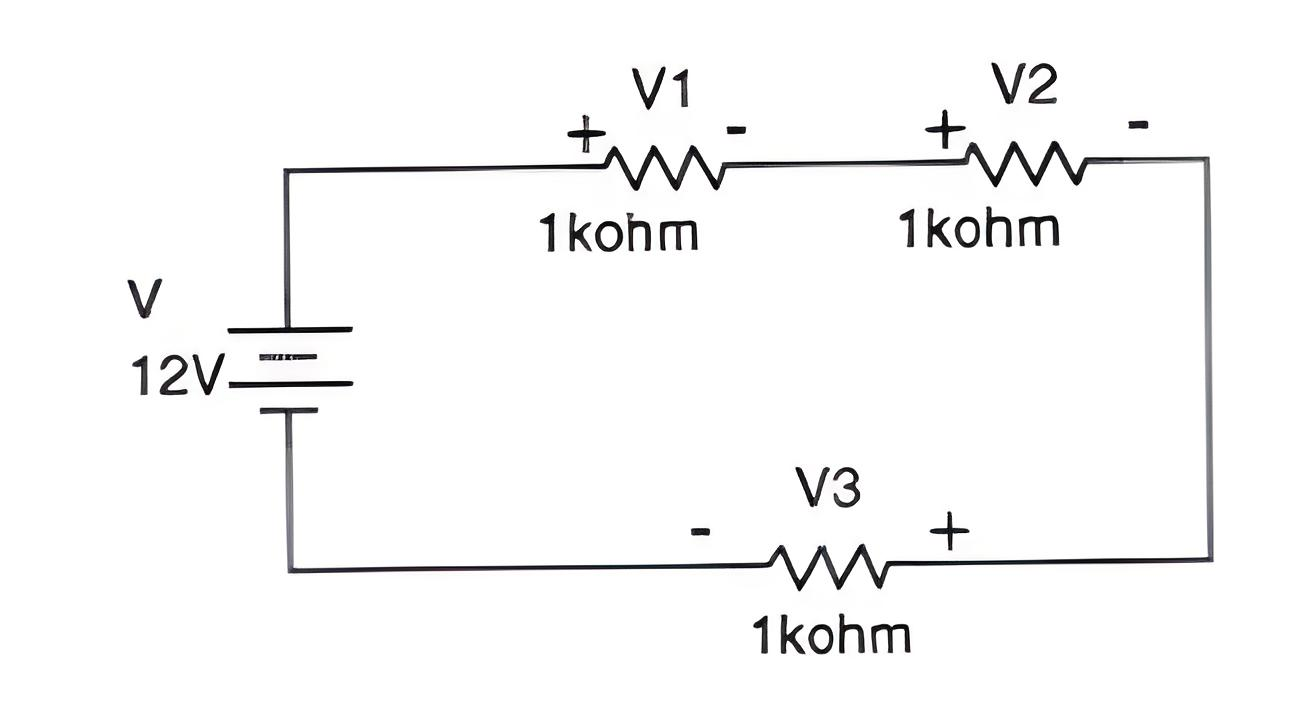
\includegraphics[scale=0.2]{imagenes/2}
	\end{figure}
	\item Verifique que la salida de la fuente PS-1 es 0 V.
	\item Conecte R5, R6, R7, R8 y la fuente de alimentación en serie, como se muestra en	la figura anterior. Luego lleve la salida de PS-1 a 8 V.
	\\
	\textbf{Nota: } Ud. ahora demostrará la ley de las tensiones de Kirchhoff midiendo las
	caídas de tensión en cada componente de la malla consistente en RS, R6, R7 y
	R8: y la fuente PS-1.\\
	
	Para trabajar correctamente con la LVK debemos realizar las mediciones de las
	caídas de tensión en la misma dirección en todo momento.\\
	
	Trabaje en dirección horaria, y siempre realice la medición con el terminal (+) del
	multímetro conectado al lado del componente que se encuentra primero en el
	movimiento horario alrededor de la malla.
	 
	\item Comience la medición seleccionando en el multímetro la escala de tensiones de
	CC. Conecte el terminal (+) del multímetro al lado izquierdo de RS, y el (-) en el
	lado derecho de R5. Mida la caída de tensión, cuidando de observar si esta es (+)
	o (-)
	\\ Continúe con cada resistor en la malla, siempre conectando el lado (+) del
	medidor primero. Finalmente mida la tensión de la fuente de alimentación, para
	completar la malla (la cual será una lectura (-).
	\\
	\\
	\\
	\begin{figure}[h]
		\centering
		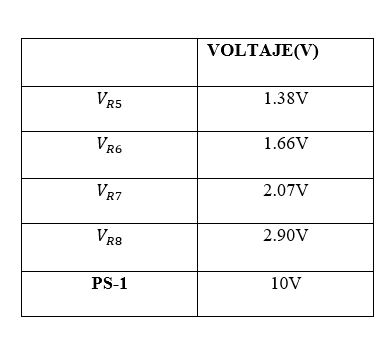
\includegraphics[scale=1.2]{imagenes/2.1}
	\end{figure}
	
	\item Sume algebraicamente (es decir, tomando en cuenta el signo) las caídas de tensión.\\
	La suma de las caídas en la malla: $V_{R5}+V_{R6}+V_{R7}+V_{R8}+PS-1= -1.38-1.66-2.07-2.90+10=0$
	\item Estudie el circuito que se muestra en la siguiente figura, observando la polaridad de las fuentes de alimentación. Lleve la salida de ambas fuentes a 0V
	\begin{figure}[h]
		\centering 
		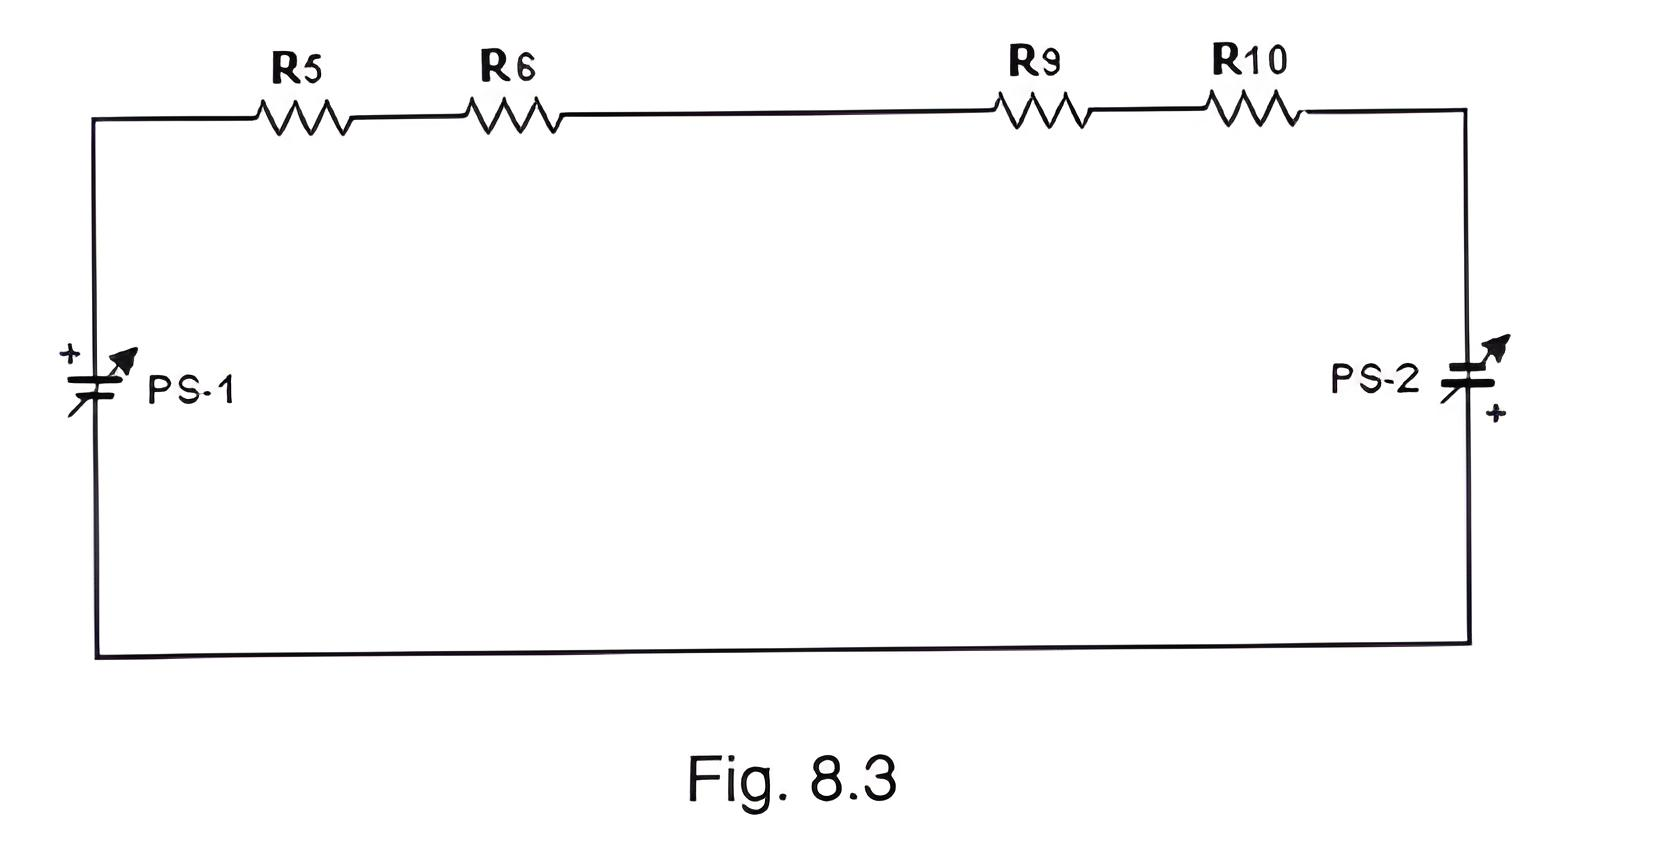
\includegraphics[scale=0.2]{imagenes/3}
	\end{figure}
	\item Conecte el circuito como se muestra en la figigura anterior
	\item Ubique las salidas de la fuentes PS-1 en 6 voltios y la PS-2  en 3 volt.
	\item Comenzando po la izquierda de R5 y siguiendo en sentido de la agujas del reloj , mida y registre en la tabla , las tensiones alrededor de la malla formada por $R_{5},R_{6}, R_{9},R_{10}$ y las fuentes de PS-1 y PS-2.
	\begin{figure}[h]
		\centering
		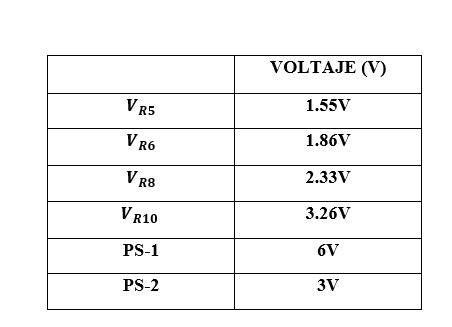
\includegraphics[scale=1.2]{imagenes/5}
	\end{figure}
	\item Sume las seis tensiones algebraicamente (valores “+” y “-“) 
	\begin{equation*}
		suma de la tensiones en la malla es -1.54V-1.86V-2.33V-3.26V+6V+3V=0 
	\end{equation*}
	\\
	Ud. ha completado el procedimiento experimental, y demostró que la suma de las caídas de tensión en una malla cerrada es cero.\\
	Aquí podrá aplicar los principios teóricos aprendidos en las actividades experimentales.
	\item Modifique el circuito de la fig. 8.2. Invierta la salida del PS-1 (PS-1 en -6 Volt y de PS-2 en -3 Volt).
	\item Comenzando por el lado izquierdo de R5 y recorriendo en sentido horario, mida e registre las tensiones alrededor de la malla. 
	\begin{equation*}
		V_{R5}= -6-3+2.33+3.26+1.86=-1.55V
	\end{equation*}
	\item Sume algebraicamente las 6 caídas de tensión (valores "+ y "-“)
	\begin{equation*}
		V_{R5}+V_{R6}+V_{R8}+V_{R10}+(PS-1)+(PS-2)= -1.54V-1.86V-2.33V-3.26V+6V+3V=0
	\end{equation*}
\end{enumerate}
\section{Autoevaluación}
\begin{enumerate}
	\item 	El valor absoluto de la suma de todas la tensiones en resistencias es:\\ 
	$1.55+1.86+3.26+2.33=9V$
	\item Dos resistencias R y 2R , son conectados en serie y estas a su vez a una batería de 12V.La tensión en los bordes de R es : 
	\begin{equation*}
		V_{R}=RI \rightarrow V_{R}=\frac{4}{R*R}=4V
	\end{equation*}
\end{enumerate}
\section{Conclusiones}
En este laboratorio se llego a usar las leyes de Kirchhoff para hallar las intenciones y los voltajes presentes en el circuito.
